\documentclass[11pt,compress,professionalfonts]{beamer}
\usetheme{metropolis}

\usepackage[]{graphicx}
\usepackage[]{color}

\usepackage{ctable}
\usepackage{hyperref}
\usepackage{dcolumn}
\usepackage{booktabs}

\usepackage{mathspec}
\setsansfont{Avenir Next}[BoldFont={* Demi Bold}]
\setmonofont[Scale = MatchLowercase,Mapping=tex-ansi]{Inconsolata}
\setmathfont(Digits,Latin,Greek){Avenir Next}
\newfontface\fancy{Avenir Light}[Mapping=tex-ansi]

\definecolor{darkgray}{rgb}{0.5,0.5,0.5}
\definecolor{darkblue}{rgb}{0.000,0.251,0.502}
\definecolor{bloodred}{rgb}{0.502,0.000,0.000}
\definecolor{darkgreen}{rgb}{0.000,0.502,0.0}
\definecolor{verylightgray}{rgb}{0.95,0.95,0.95}

\setbeamerfont{frametitle}{size=\Large,family=\fancy}
\setbeamercolor{frametitle}{fg=bloodred, bg=verylightgray}
\setbeamerfont{title}{family=\fancy,size=\Large}
\setbeamercolor{title}{fg=bloodred}
\setbeamercolor{background canvas}{bg=white}
\setbeamercolor{normal text}{fg=black}
\setbeamercolor{title separator}{fg=darkgray}

\metroset{progressbar=none,numbering=none}

\IfFileExists{upquote.sty}{\usepackage{upquote}}{}

%% bullet free bullet points
\newcommand{\ita}{\begin{itemize}}
\newcommand{\itm}{\item[]}
\newcommand{\itz}{\end{itemize}}

% graphics file in the pics subdirectory please
\graphicspath{{./pics/}}

%%%%%%%%%%%%%%%%%%%%%%%%%%%%%%%%%%%%%%%%%%%%%%%%%%%%%%%%%%%%%%%%%%%%%%%%%%%%%%%%%%%%%%%%
\title{Computer-assisted content analysis}
\author{Will Lowe ~~Princeton University \\ James Lo ~~ University of Southern California}
\date{Part 2}
\begin{document}

\maketitle

%
%How to model categorical $\theta$ without specifying a dictionary and without having a training set?
%
%Example questions:
%
%Simple case: What proportion of weblogs strongly dislike, dislike, are indifferent to, like or strongly like Kerry as a candidate?
%
%Harder case: How does the balance of topics in a corpus change over time?
%

%\slide{Topic Models 1}

%\centerline{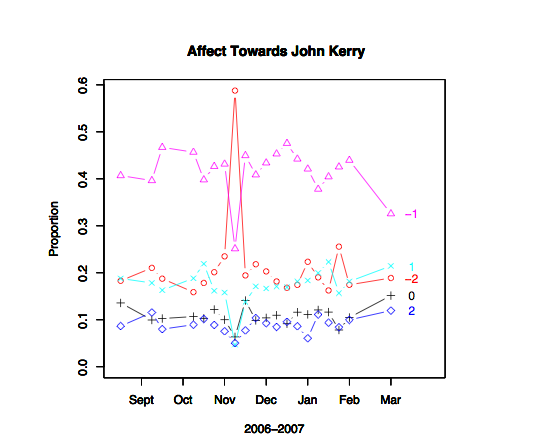
\includegraphics[scale=.8]{pictures/kerry-blogs}}
%

\begin{frame}[t,fragile]\frametitle{Menu}

Session 1: Classical Content Analysis

Session 2:
\ita
\itm Document classification
\ita
\itm The direct approach to classification
\itm The indirect approach to classification
\itm Evaluation and interpretation
\itm Topic models
\itz
\itz

Session 3: Scaling Models

\end{frame}


%\begin{frame}[t,fragile]\frametitle{Text as Data}
%\centerline{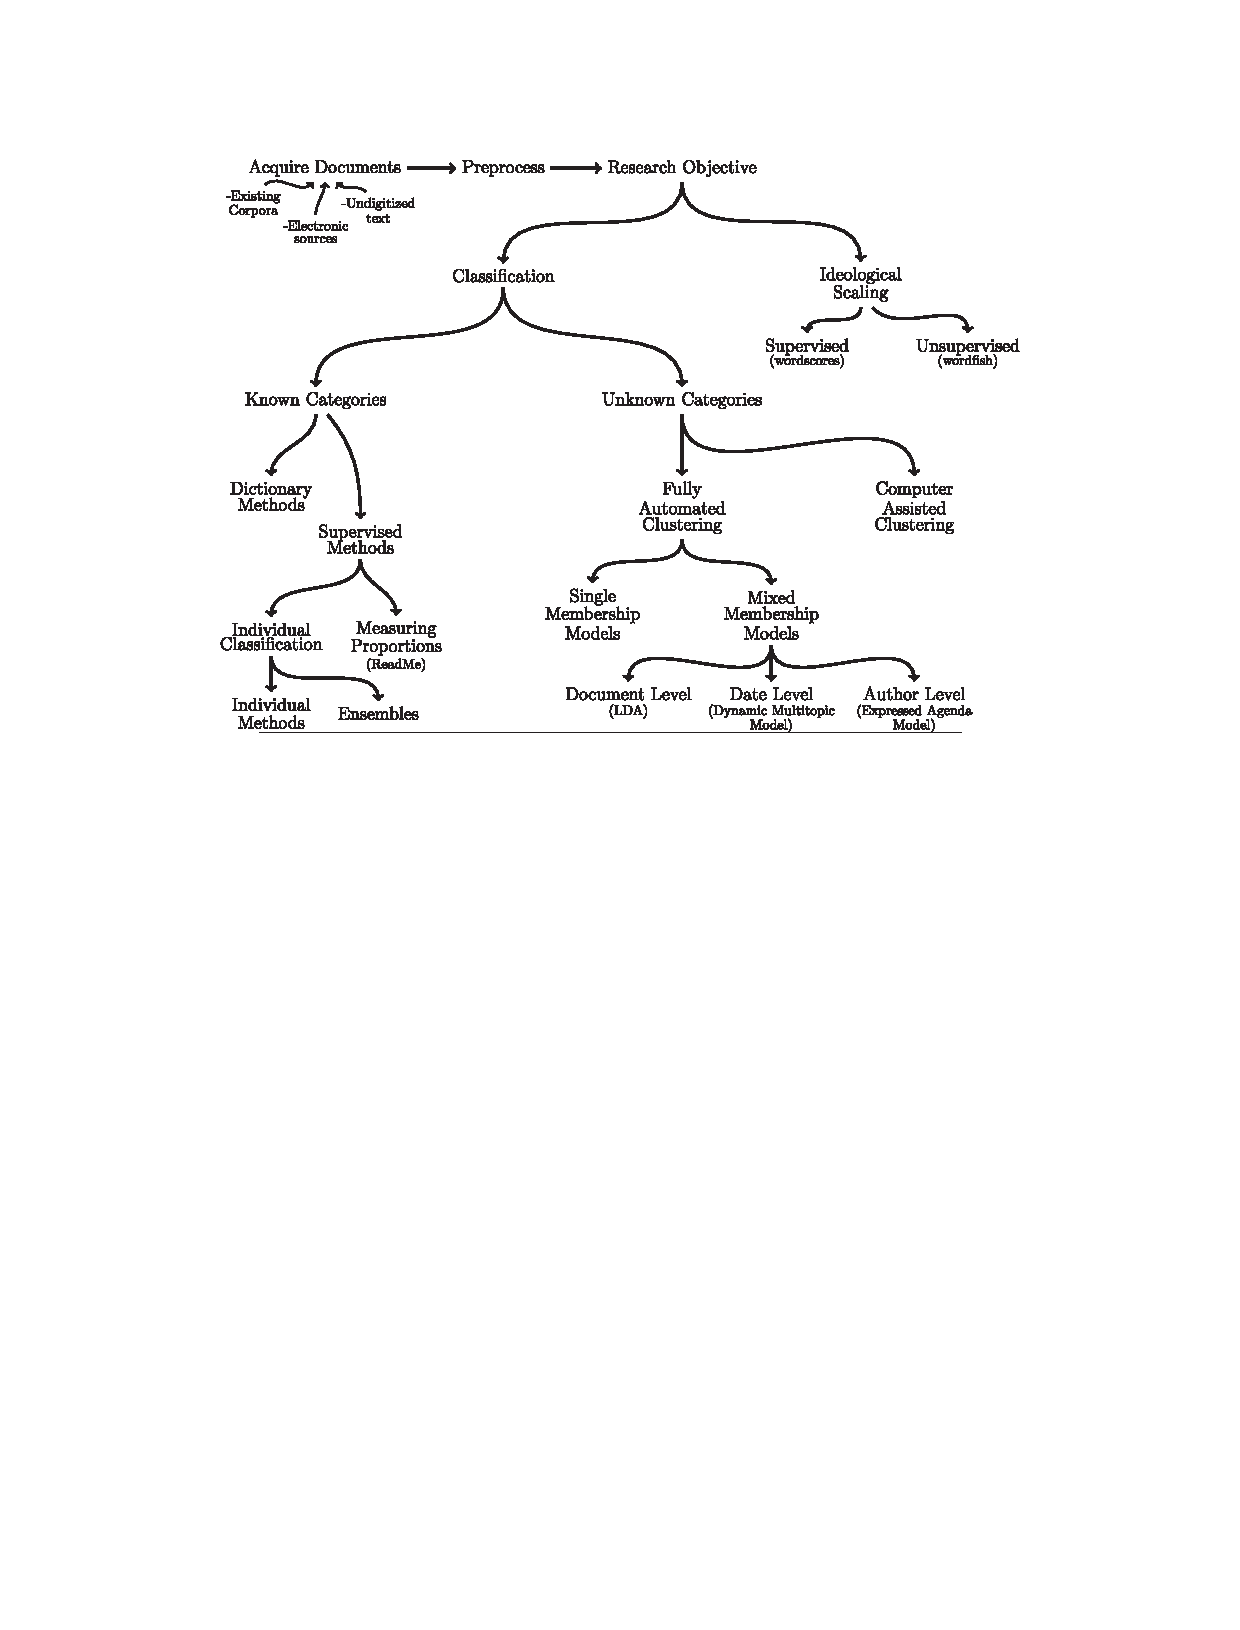
\includegraphics[scale=.7]{pictures/grimmerovreview.pdf}}
%\centerline{\footnotesize Source: Grimmer and Stewart (2013)}
%\end{frame}


%%%%%%%%%%%%%%%%
%%%%%%%%%%%%%%%%


\begin{frame}[t,fragile]\frametitle{Classification Approaches when Categories are Known}

We often want to read text to put them into categories

{\bf Examples:}

\begin{enumerate}
\item Are campaign advertisements positive or negative?
\item What policy areas do newspaper editorials cover?
\item Are international statements belligerent or peaceful?
\item Do court letters liberal or conservative?
\item Is this email spam?
\end{enumerate}


\end{frame}



\begin{frame}[t,fragile]\frametitle{Classification}
\vspace{10 mm}
\centerline{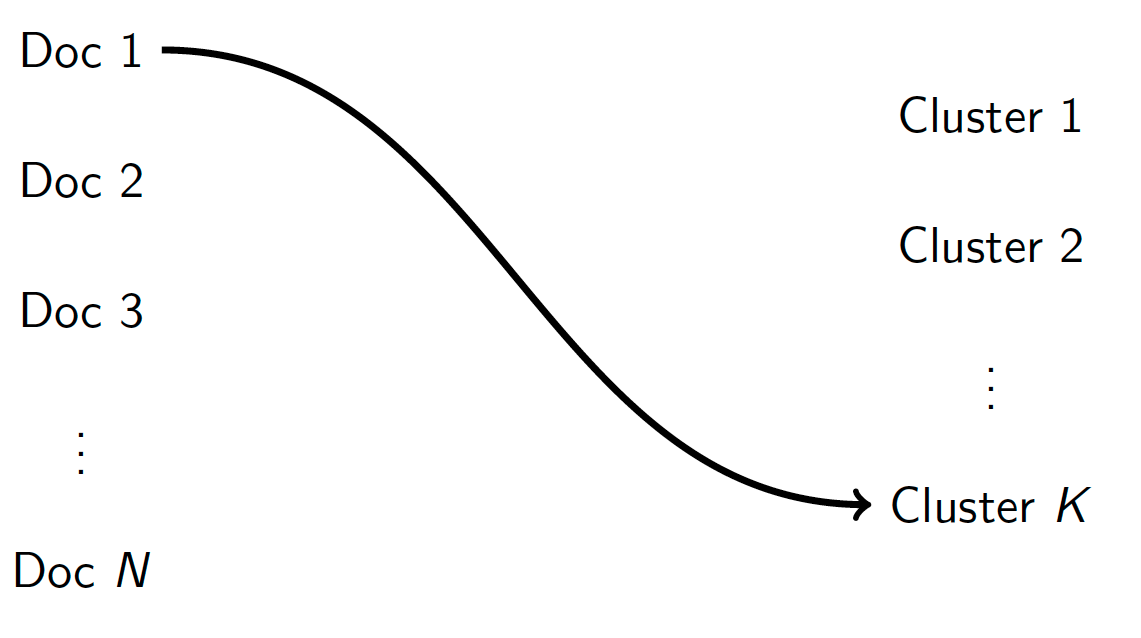
\includegraphics[scale=.2]{pictures/classification.png}}
\centerline{\normalsize For classification, each document belongs to a single cluster}
\end{frame}

\begin{frame}[t,fragile]\frametitle{Topic Models}
\vspace{10 mm}
\centerline{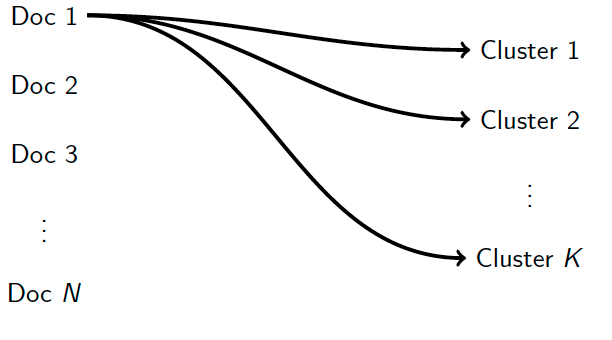
\includegraphics[scale=.4]{pictures/LDA.png}}
\centerline{\normalsize In LDA, each document can contain multiple topics}
\end{frame}


\begin{frame}[t,fragile]\frametitle{Classification Approaches when Categories are Known}

{\bf Yesterday:} Classification using dictionary approach.

An alternative is \textbf{supervised machine learning} methods:
\begin{enumerate}

\item coders categorize a set of documents by hand
\item the algorithm ``learns'' how to sort the documents in categories
\item  characteristics of training set are used  to assign new documents to categories.
\end{enumerate}
\ita
\itm Naive Bayes, Maximum Entropy, Support Vector Machines, Neural Networks, Bagging, Boosting, $\ldots$
\itz
\end{frame}

\begin{frame}[t,fragile]\frametitle{Classification Approaches when Categories are Known}

Let $\theta_k$ be the \textit{probability} that Z=k for each document
\ita
\itm Words are denoted $\{W\}$
\itm Each document has a \textit{single} topic Z
\itm Some topic labels are observed
\itm We essentially want $P(Z \mid \{W\}) = \theta_{z|w}$
\itz
\vfill
Supervised machine learning
\ita
\itm Tries to give good predictions of observed Y given X
\itm Naive Bayes, Maximum Entropy, Support Vector Machines, Neural Networks, Bagging, Boosting, $\ldots$
\itz
\end{frame}


%We can \textit{choose} a style of model\\
%~\\
%\centerline{\includegraphics[scale=.7]{pictures/classification-plate}~~~~~~~~~
%\includegraphics[scale=.7]{pictures/classification-plate2}}

%\centerline{Discriminative Style ~~~~~~~~~~~~~~~~ Generative Style}



%\begin{frame}[t,fragile]\frametitle{Classification Approaches}
%Much of machine learning, computational linguistics, and AI deals with classification problems
%Methods:
%\ita
%\itm Naive Bayes, Maximum Entropy, Support Vector Machines, Neural Networks, Bagging, Boosting, $\ldots$
%\itm We only touch on the issues here\ldots
%\itz
%\end{frame}

%\begin{frame}[t,fragile]\frametitle{Classification approaches}
%In the simple framework of yesterday
%\ita
%\itm $Z$ is the true category of a document
%\itm $\theta$ is be the posterior probability that a document is a particular category
%\itz
%\end{frame}


\begin{frame}[t,fragile]\frametitle{Classification approaches}
As before, we have two approaches
\ita
%\itm Discriminative: Model $P(Z \mid \{W\}, \beta) = \theta_{z|w}$ directly
%\itm Generative: Model $P(\{W\} \mid Z, \beta)$ and $P(Z)=\theta_z$, then get $P(Z \mid \{W\}, \beta) = \theta_{z|w}$ via Bayes theorem
\itm Discriminative: Model $P(Z \mid \{W\}) = \theta_{z|w}$ directly
\itm Generative: Model $P(\{W\} \mid Z)$ and $P(Z)=\theta_z$, then get $P(Z \mid \{W\}) = \theta_{z|w}$ via Bayes theorem
\itz
\vfill
\textbf{Bayes theorem} is about inverse probabilities
\ita
%\itm Suppose you know $P(\{W\} \mid Z)$
%\itm We can (sometimes) say something about $P(Z \mid \{W\} )$
\itm $P(A | B) = \frac{P(B | A) P(A)}{P(B)}$
\itm If $P(\{W\} \mid Z)$ known, estimate $P(Z \mid \{W\} )$
\itz
\end{frame}



%\begin{frame}[t,fragile]\frametitle{Generative vs discriminative training}
%\centerline{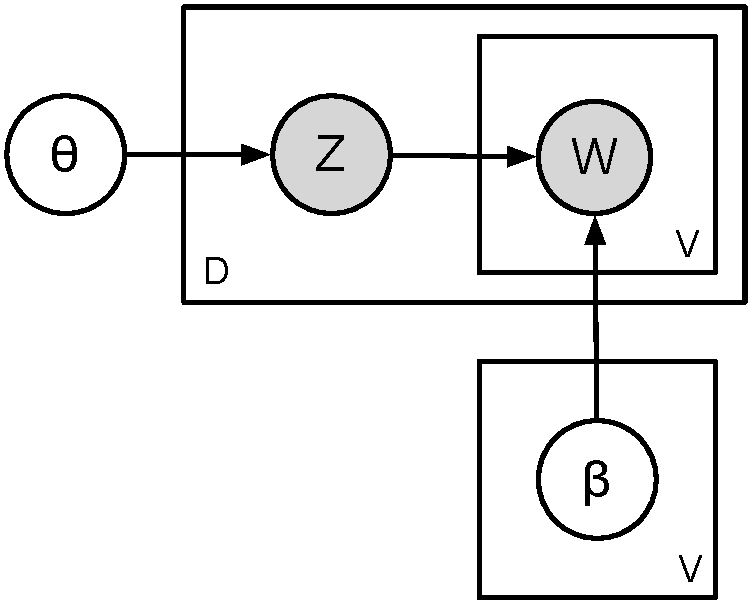
\includegraphics[scale=.4]{pictures/unsupervised-classification} \hfill \includegraphics[scale=.4]{pictures/supervised-%classification}}
%Naive Bayes \hfill Maximum Entropy, etc...
%\vfill
%\end{frame}

%\begin{frame}[t,fragile]\frametitle{Generative vs discriminative testing}
%\centerline{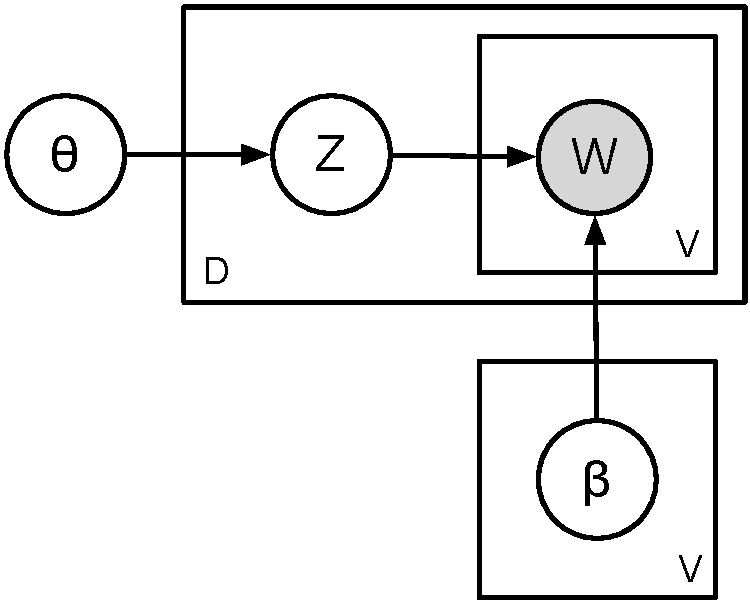
\includegraphics[scale=.4]{pictures/unsupervised-classification-test} \hfill 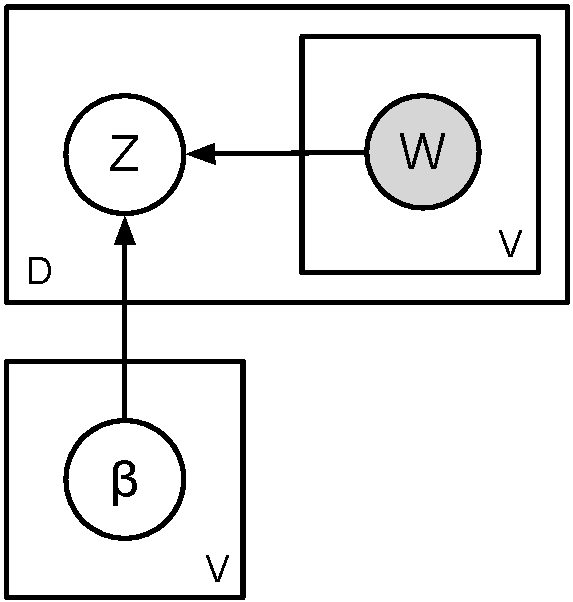
\includegraphics[scale=.4]{pictures/supervised-classification-test}}
%Naive Bayes \hfill Maximum Entropy, etc...
%\end{frame}


\begin{frame}[t,fragile]\frametitle{Either way\ldots}

Desirable classification outcome:

\begin{center}
\begin{tabular}{lcc}
& $P(Z=`\text{Domestic}'\mid \{W\}_d)$ & $P(Z=`\text{Foreign}' \mid \text \{W\}_d)$ \\ \toprule
$D_1$ & 0.75 & 0.25 \\
$D_2$ & 0.82 & 0.18 \\
\ldots & \ldots & \ldots\\
$D_{N-1}$ & 0.02 & 0.98 \\
$D_N$ & 0.45 & 0.55\\ \bottomrule
\end{tabular}
\end{center}

where $\theta_{z|w} = P(Z=z \mid \{W\})$

\end{frame}


\begin{frame}[t,fragile]\frametitle{The Basic Steps}
\begin{enumerate}
\item Construct a training set
(a) create a coding scheme\\
(b) select documents (ideally randomly sampled)
\item Apply the supervised learning method to learn features of a training set and infer labels
\item Validate and classify remaining documents\\
\end{enumerate}
We will do this in the lab together with NY Times titles
\end{frame}


\begin{frame}[t,fragile]\frametitle{An Applied Example: Affirmative Action}
Evans et al. (2007) apply naive Bayes to legal text
\ita
\itm Affirmative action programs at university level
\itz
Examine Amicus Curiae briefs sent to appellate court
\ita
\itm Can words tell us direction of AC brief?
\itm Are the briefs liberal or conservative?
\itz


\end{frame}



%\begin{frame}[t,fragile]\frametitle{Indirect approach: Naive Bayes}
%Background:
%\ita
%\itm Amicus Curiae (friend of the court) briefs are submitted to an appellate court
%\itm They usually present a legal argument for or against one of the parties to a case
%\itm Amicus Curiae can be submitted by any group that feels that it has a stake in the case
%\itz
%\end{frame}
%\begin{frame}[t,fragile]\frametitle{Affirmative action}
%Evans et al. use cases about the constitutionality of `affirmative action' programs at university level
%\ita
%\itm Regents of the University of California vs. Bakke (1978)
%\itm Grutter vs Bollinger, Lehman, Shields, and the Regents of the University of Michigan (2003)
%\itm Gratz and Hamacher vs Bollinger, Lehman, Shields and the Regents of the University of Michigan (2003)
%\itz
%The arguments are as much \textsl{political} (state vs federal rights, social welfare, constitutional interpretation) as they are \textsl{legal}
%\end{frame}
%\begin{frame}[t,fragile]\frametitle{Affirmative Action}
%This work uses document classification to answer two questions
%\ita
%\itm To what extent can the \textsl{direction} of an AC brief be predicted on the basis of its words?
%\itm What can we learn about \textsl{language} of each side of the case?
%\itz
%\end{frame}


\begin{frame}[t,fragile]\frametitle{Naive Bayes}

\textsl{Naive Bayes} is a relatively old ($\sim$1975)  classification method

Want to guess if document $j$ is liberal/conservative based on its word profile $\{W\}_j$.

Probability can be derived by applying Bayes theorem:

\begin{align*}
P(A | B) &= \frac{P(B | A) P(A)}{P(B)}\\
P(Z=\text{`Lib'} \mid \{W\}_j) &~=~ \frac{P(\{W\}_j \mid Z=\text{`Lib'})~P(Z=\text{`Lib'})}{P(\{W\}_j)}
\end{align*}

\end{frame}
\begin{frame}[t,fragile]\frametitle{Naive Bayes}

\begin{align*}
P(Z=\text{`Lib'} \mid \{W\}_j) &~\propto~ P(\{W\}_j \mid Z=\text{`Lib'})~P(Z=\text{`Lib'})
\end{align*}

We can drop $P(\{W\}_j)$ since it is constant across categories.

Given a representative training set, estimating $P(Z=L)$ is easy:

\begin{align*}
\hat{P}(Z=\text{`Lib'})&~=~ \frac{\text{\# training docs that are liberal}}
{\text{\# of training docs}}
\end{align*}

\end{frame}
\begin{frame}[t,fragile]\frametitle{Naive Bayes}

Estimating the probability that a word profile $\{W\}_j$ occurs given that the document is liberal $P(\{W\}_j\mid Z=\text{`Lib'})$ is more challenging, because any one word profile is likely to occur only once.

Assumption: words are assumed to be generated \textit{independently} given the category Z 
\begin{align*}
P(\{W\}_j \mid Z=\text{`Lib'}) &~=~ {\prod}_i P(W_i \mid Z=\text{`Lib'})\\
P( \text{`Affirmative Action'} \mid Z=\text{`Lib'}) &~=~ P( \text{`Affirmative'} \mid Z=\text{`Lib'}) \cdot\\
& ~  P( \text{`Action'} \mid Z=\text{`Lib'})
\end{align*}


\end{frame}



\begin{frame}[t,fragile]\frametitle{Naive Bayes}

With this assumption, we can estimate the probability of observing a word $i$  given that the document is liberal: proportion of word $i$ in liberal training set.

The classifier then chooses the class Z (Liberal or Conservative) with the highest aggregate probability.

Note that every new word adds a bit of information that re-adjusts the conditional probabilities.

\newpage


\end{frame}
\begin{frame}[t,fragile]\frametitle{Naive Bayes}



Note that with two classes (here: liberal and conservative)  this has a rather neat interpretation:
\begin{align*}
\frac{P(Z=\text{\text{`Lib'}} \mid \{W\}_j)}
{P(Z=\text{`Con'} \mid \{W\}_j)} = \\
~~~~~~~~~\prod_i \frac{P(W_i \mid Z=\textsl{\text{`Lib'}})}
{P(W_i \mid Z=\textsl{`Con'})}\times \frac{P(Z=\textsl{\text{`Lib'}})}{~P(Z=\textsl{`Con'})}
\end{align*}
Logging this probability ratio, every new word \textsl{adds} a bit of information that pushes the ratio above or below 0

%%%%%%%%%%% check the below works in the real document

%[will@Apparent lib]$ ykcats -dictionary ../../disc.vbpro ../lib/*
%,Dictionary,Dictionary>discrimination,WordCount
%6019_ll01-utf8.txt,26,26,20002
%6020_ll01-utf8.txt,13,13,18722
%[will@Apparent lib]$ ykcats -dictionary ../../disc.vbpro ../con/*
%,Dictionary,Dictionary>discrimination,WordCount
%6019_lc01-utf8.txt,70,70,17368
%6020_lc01-utf8.txt,48,48,17698

% lib = (26+13)/(20002+18722) = 0.001007127
% con = (70+48)/(17368+17698) = 0.003365083
% lib / con = .299

%%%%%%%%%%%

\end{frame}
\begin{frame}[t,fragile]\frametitle{Naive Bayes}

Example: Naive Bayes with only word class `discriminat*'.
{\small
\begin{align*}
P(W=\text{`discriminat*'} \mid Z=\text{`Lib'}) & = (26+13)/(20002+18722) \approx 0.001\\
P(W=\text{`discriminat*'} \mid Z=\text{`Con'}) & = (70+48)/(17368+17698) \approx 0.003
\end{align*}
}
Assume that liberal and conservative supporting briefs are equally likely (true in the training set)
\begin{align*}
\frac{P(Z=\text{\text{`Lib'}})}{P(Z=\text{`Con'})} & = 1
\end{align*}

Last step:  calculate posterior classification  probabilities for a new document (based on occurrence of this word).

\end{frame}
\begin{frame}[t,fragile]\frametitle{Naive Bayes}

%(File 6019\_al18-utf8.txt)
Amicus brief from `King County Bar Association' containing 3667 words and 4 matches to disciminat*.

{\scriptsize
\begin{verbatim}
that "the state shall not [discriminate] against, or grant preferential treatment
the lingering effects of racial [discrimination] against minority groups in this
remedy the effects of societal [discrimination]. Another four Justices (Stevens
that "the state shall not [discriminate] against, or grant preferential treatment
\end{verbatim}
}
\end{frame}


\begin{frame}[t,fragile]\frametitle{Naive Bayes}
A priori, the probabilities are\ldots

Probability that we observe the word  discriminat* 4 out of 3667 times if the document is liberal:
{\small
\begin{verbatim}
> dbinom(4, size=3667, prob=0.001007127)
[1] 0.1930602
\end{verbatim}
}
Probability that we observe the word  discriminat* 4 out of 3667 times if the document is conservative:
{\small
\begin{verbatim}
> dbinom(4, size=3667, prob=0.003365083)
[1] 0.004188261
\end{verbatim}
}
Logged probability ratio = 3.83
\newpage
\end{frame}


\begin{frame}[t,fragile]\frametitle{Naive Bayes}

Conclusion: Seeing 4 instances of discriminat* gives the posterior classification probabilities
\ita
\itm $\theta_\text{liberal} = \frac{0.193}{0.193+0.004}$ = 0.979
\itm $\theta_\text{conservative}$ =  1-0.979=0.021
\itz

This is \textit{quite} confident
\ita
\itm \ldots but other words will be less loaded or push the other way
\itz
\end{frame}



%\begin{frame}[t,fragile]\frametitle{Evaluating Classifiers: Accuracy, Precision and Recall}
%How can we evaluate how good a supervised classifier works?
%Use the confusion matrix (training set versus machine)
%\end{frame}


\begin{frame}[t,fragile]\frametitle{Evaluating Classifiers: Accuracy, Precision and Recall}

\begin{center}
\scalebox{0.8}{
\begin{tabular}{llcc}
\toprule
&&\multicolumn{2}{c}{Machine}\\
\cline{3-4}
&& Liberal & Conservative \\
\midrule
Training Data & Liberal & 40&10\\
& Conservative &40&60\\
\bottomrule
\end{tabular}}
\end{center}

\vspace*{0.5cm}

Accuracy = (40+60)/150 = .66

Precision ($Z_{machine}$=Liberal) = 40/(40+40) = 0.5

Precision ($Z_{machine}$=Cons) = 60/(10+60) = 0.86

Recall ($Z_{training}$=Liberal) = 40/(40+10) = 0.80

Recall ($Z_{training}$=Cons) = 60/(40+60) = 0.60

%\newpage
%\centerline{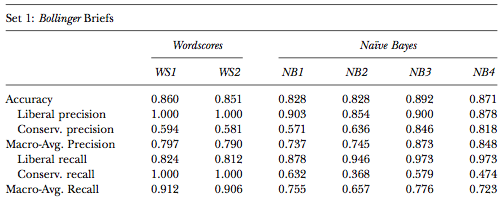
\includegraphics[scale=.9]{pictures/bolinger}}

\end{frame}


%\begin{frame}[t,fragile]\frametitle{Trading off precision and recall}
%\centerline{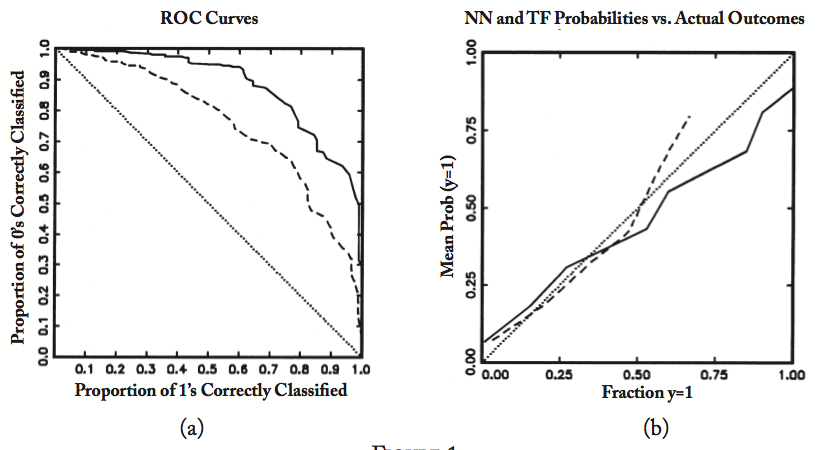
\includegraphics[scale=.4]{pictures/roc-curves}}
%(King and Zeng, 2001)
%\end{frame}
%\begin{frame}[t,fragile]\frametitle{Evaluation}
%All classification models have a secret extra parameter: the \textit{threshold}
%\end{frame}


%\begin{frame}[t,fragile]\frametitle{Distinctive Words}
%Detecting different rhetorical styles of liberal and conservative groups:
%``Liberal groups use language emphasizing the impact of affirmative action polices, while conservative words indicate concern over legal-constitutional limits on administrative procedure'' (Evans et al. 2007, p. 1029)
%\newpage
%\end{frame}

%\centerline{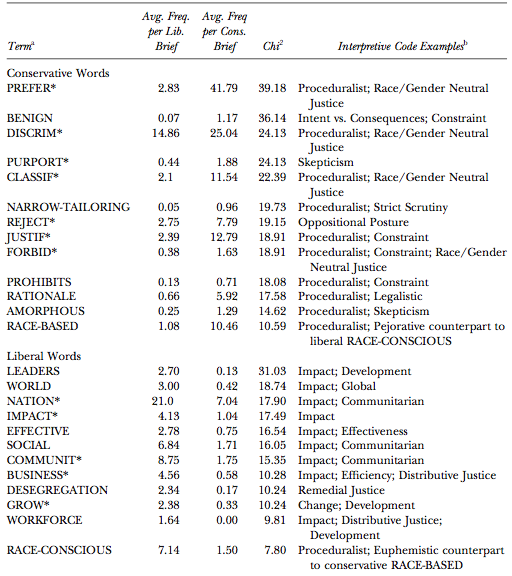
\includegraphics[scale=.6]{pictures/words-evans}}
%
%\slide{Refresher on $\chi^2$}
%
%A $\chi^2$ \textsl{statistic} is computed as
%\begin{align*}
%\frac{(\text{observed} - \text{expected})^2}{\text{expected}}
%\end{align*}
%In large samples it has a $\chi^2$ \textsl{distribution}.
%
%For measuring how useful a term would be in a classifier we are more interested in magnitude
%
%
%\slide{Refresher on $\chi^2$}
%
%\begin{center}
%\begin{tabular}{llll}
%            & purport* & not purport*   & \\ \midrule
%petitioners & 43       & 166101       & 166144 \\
%respondents & 34       & 673552       & 673586 \\ \midrule
%            & 77       & 839653       & 839730
%\end{tabular}
%\end{center}
%
%If purport* words occurred at the \textsl{same} rate then their expected proportion would be
%\[
%\frac{77}{839730}
%\]
%
%
%If \textit{not} we would estimate the rates as
%\begin{align*}
%\text{conservatives:} && \frac{43}{166144}\\
%\text{liberals:} && \frac{34}{673586}
%\end{align*}
%
%
%The $\chi^2$ asks whether the observed counts are probable under the assumption that words occur at the \textsl{same} rate. Conservatives use purport* words at more than 5 times the rate of liberals.\\
%\begin{align*}
%\frac{43~/~166144}{34~/~673586} & = 5.127
%\end{align*}
%
%\newpage
%Evans et al. 2007: "Many conservatives doubt that diversity is "narrowly tailored" to achieve a compelling state interest as "purported," or that it actually delivers many of its "alleged" benefits." (p.1030)
%
%
%\newpage
%\centerline{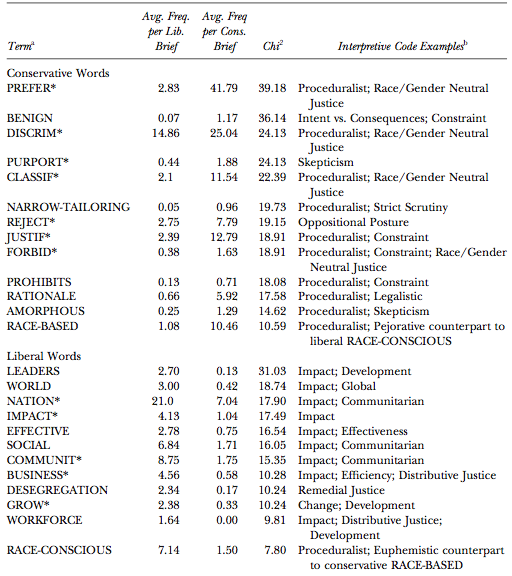
\includegraphics[scale=.9]{pictures/words-evans}}



%\begin{frame}[t,fragile]\frametitle{Compare and Contrast}
%Bara et al. (2007) abortion debate with a thematic dictionary
%\begin{center}
%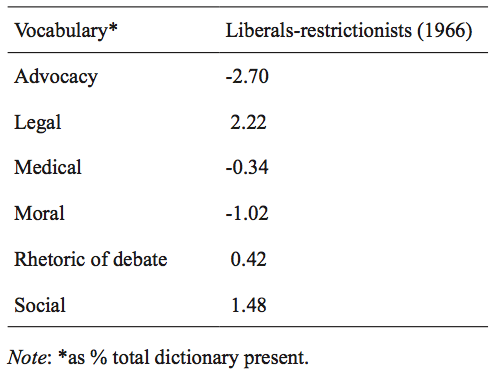
\includegraphics[scale=.4]{pictures/bara-diffs}
%\end{center}
%\end{frame}

%\begin{frame}[t,fragile]\frametitle{Vocabulary Usage}
%We can use known Z to characterize vocabulary usage directly, if we're careful\ldots
%Monroe et al. (2008) compare different measures of `partisan vocabulary' in abortion debates
%\ita
%\itm Simple frequencies will be misleading
%\itm They settle for Laplace regularized odds-ratios
%\itz
%\newpage
%\centerline{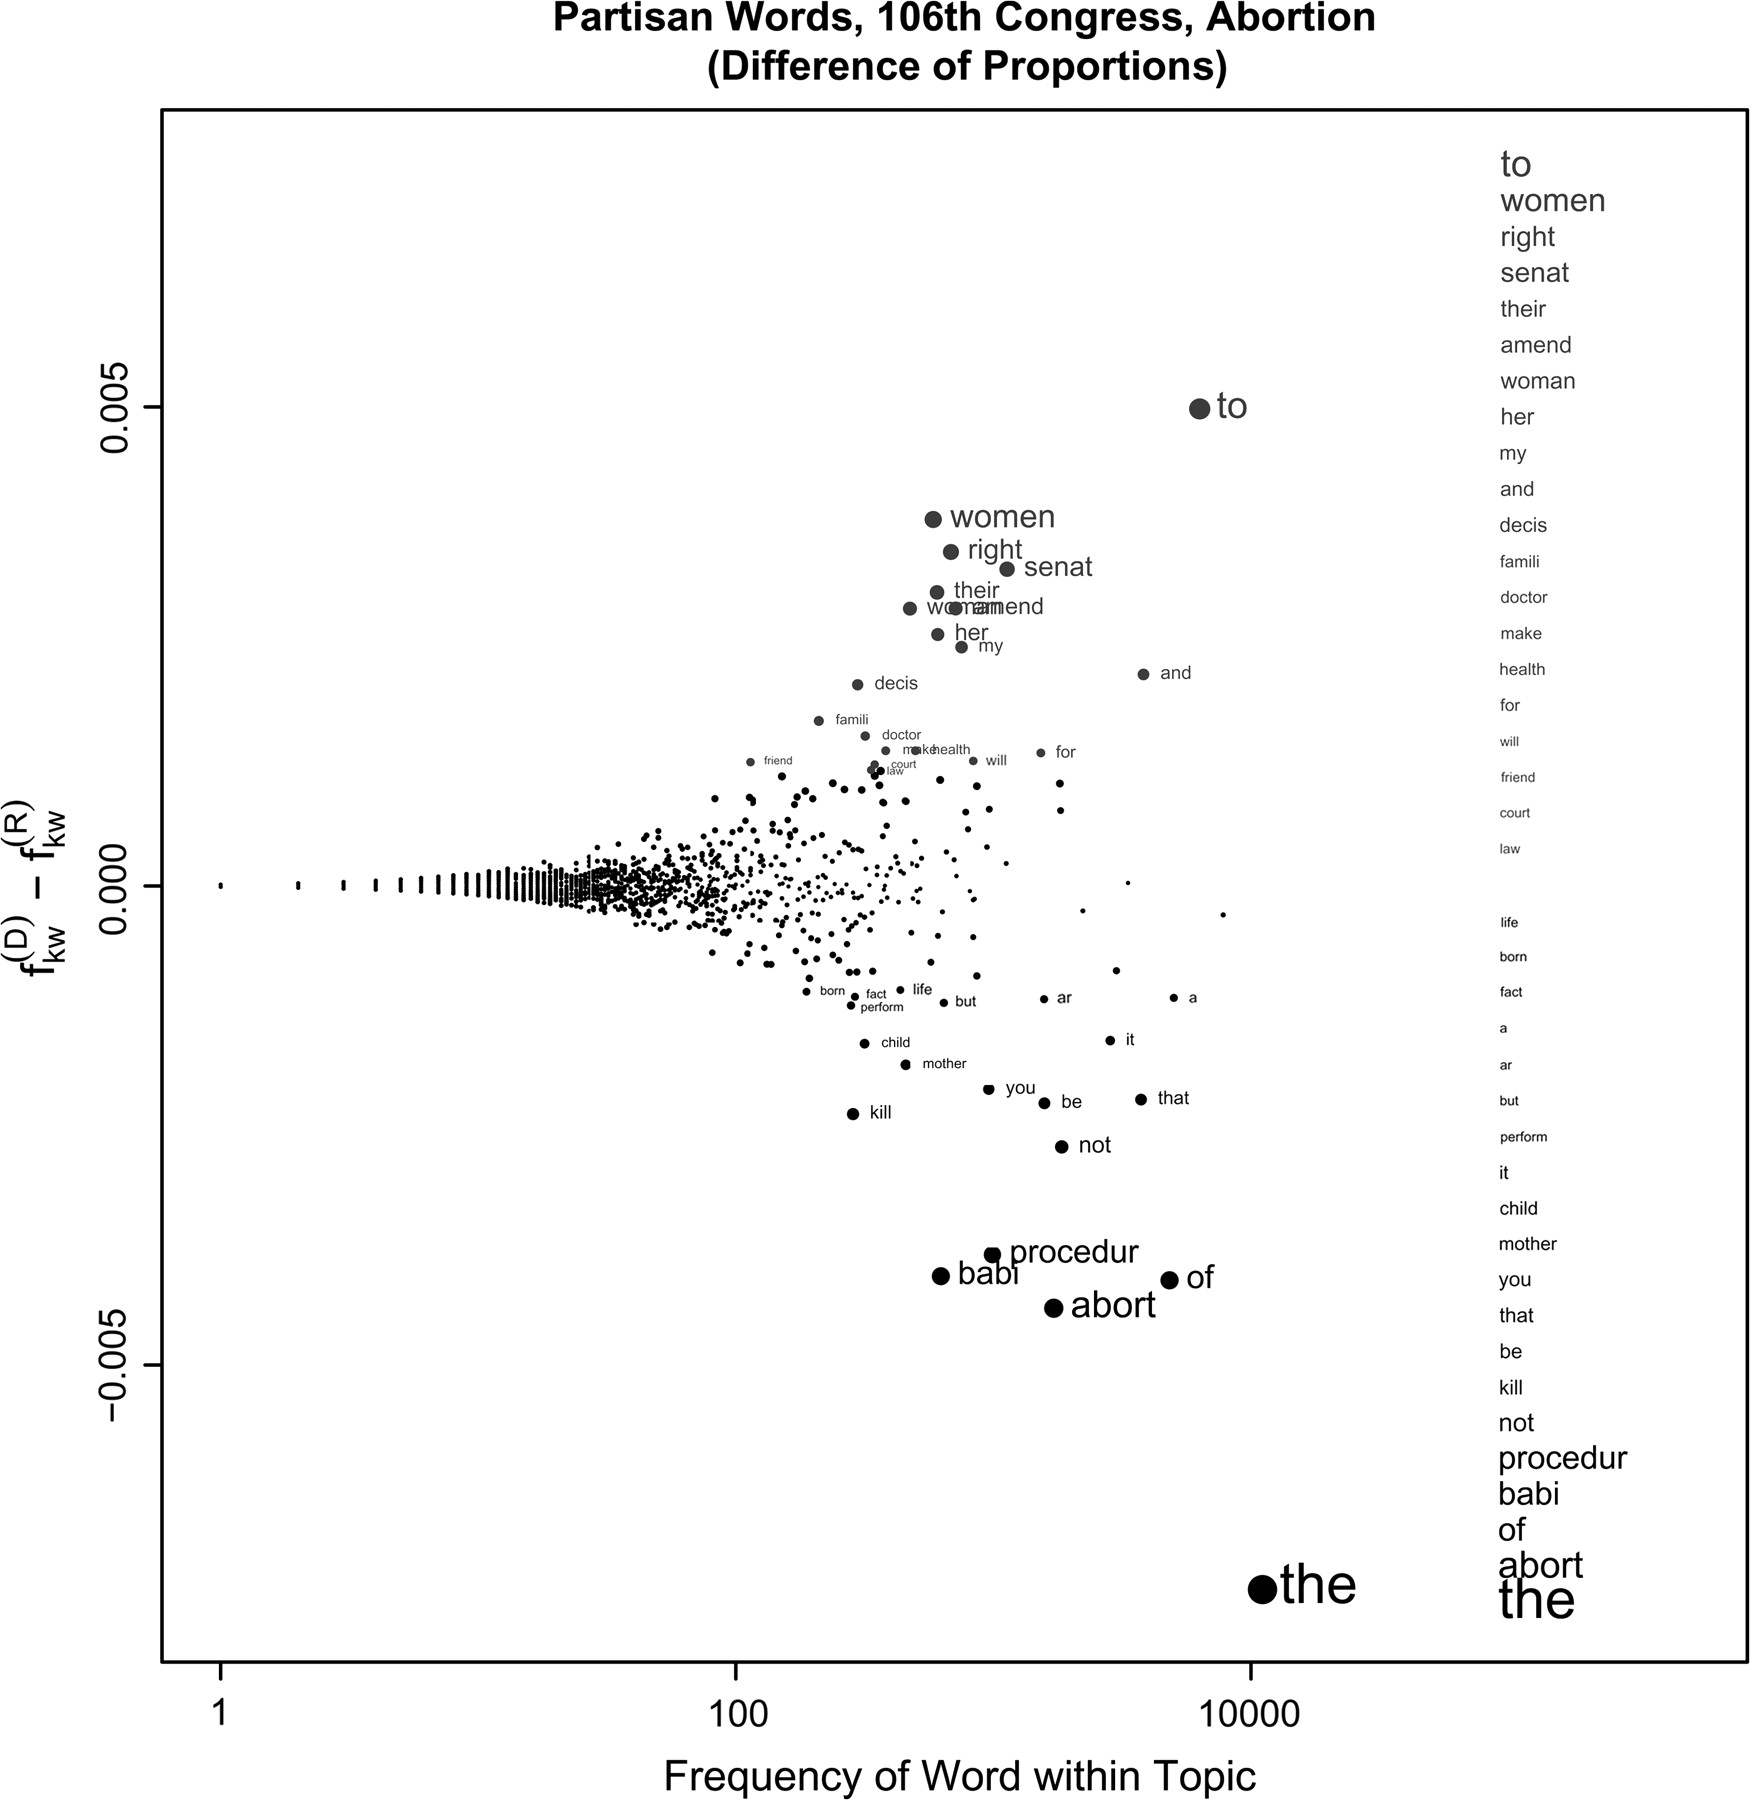
\includegraphics[scale=.1]{pictures/fightin0}}
%{\footnotesize Difference of proportions: could result in lack of overall semantic validity due to the overemphasis on high-frequency words, unclear which words matter (Monroe et al. 2009).}
%\newpage
%\centerline{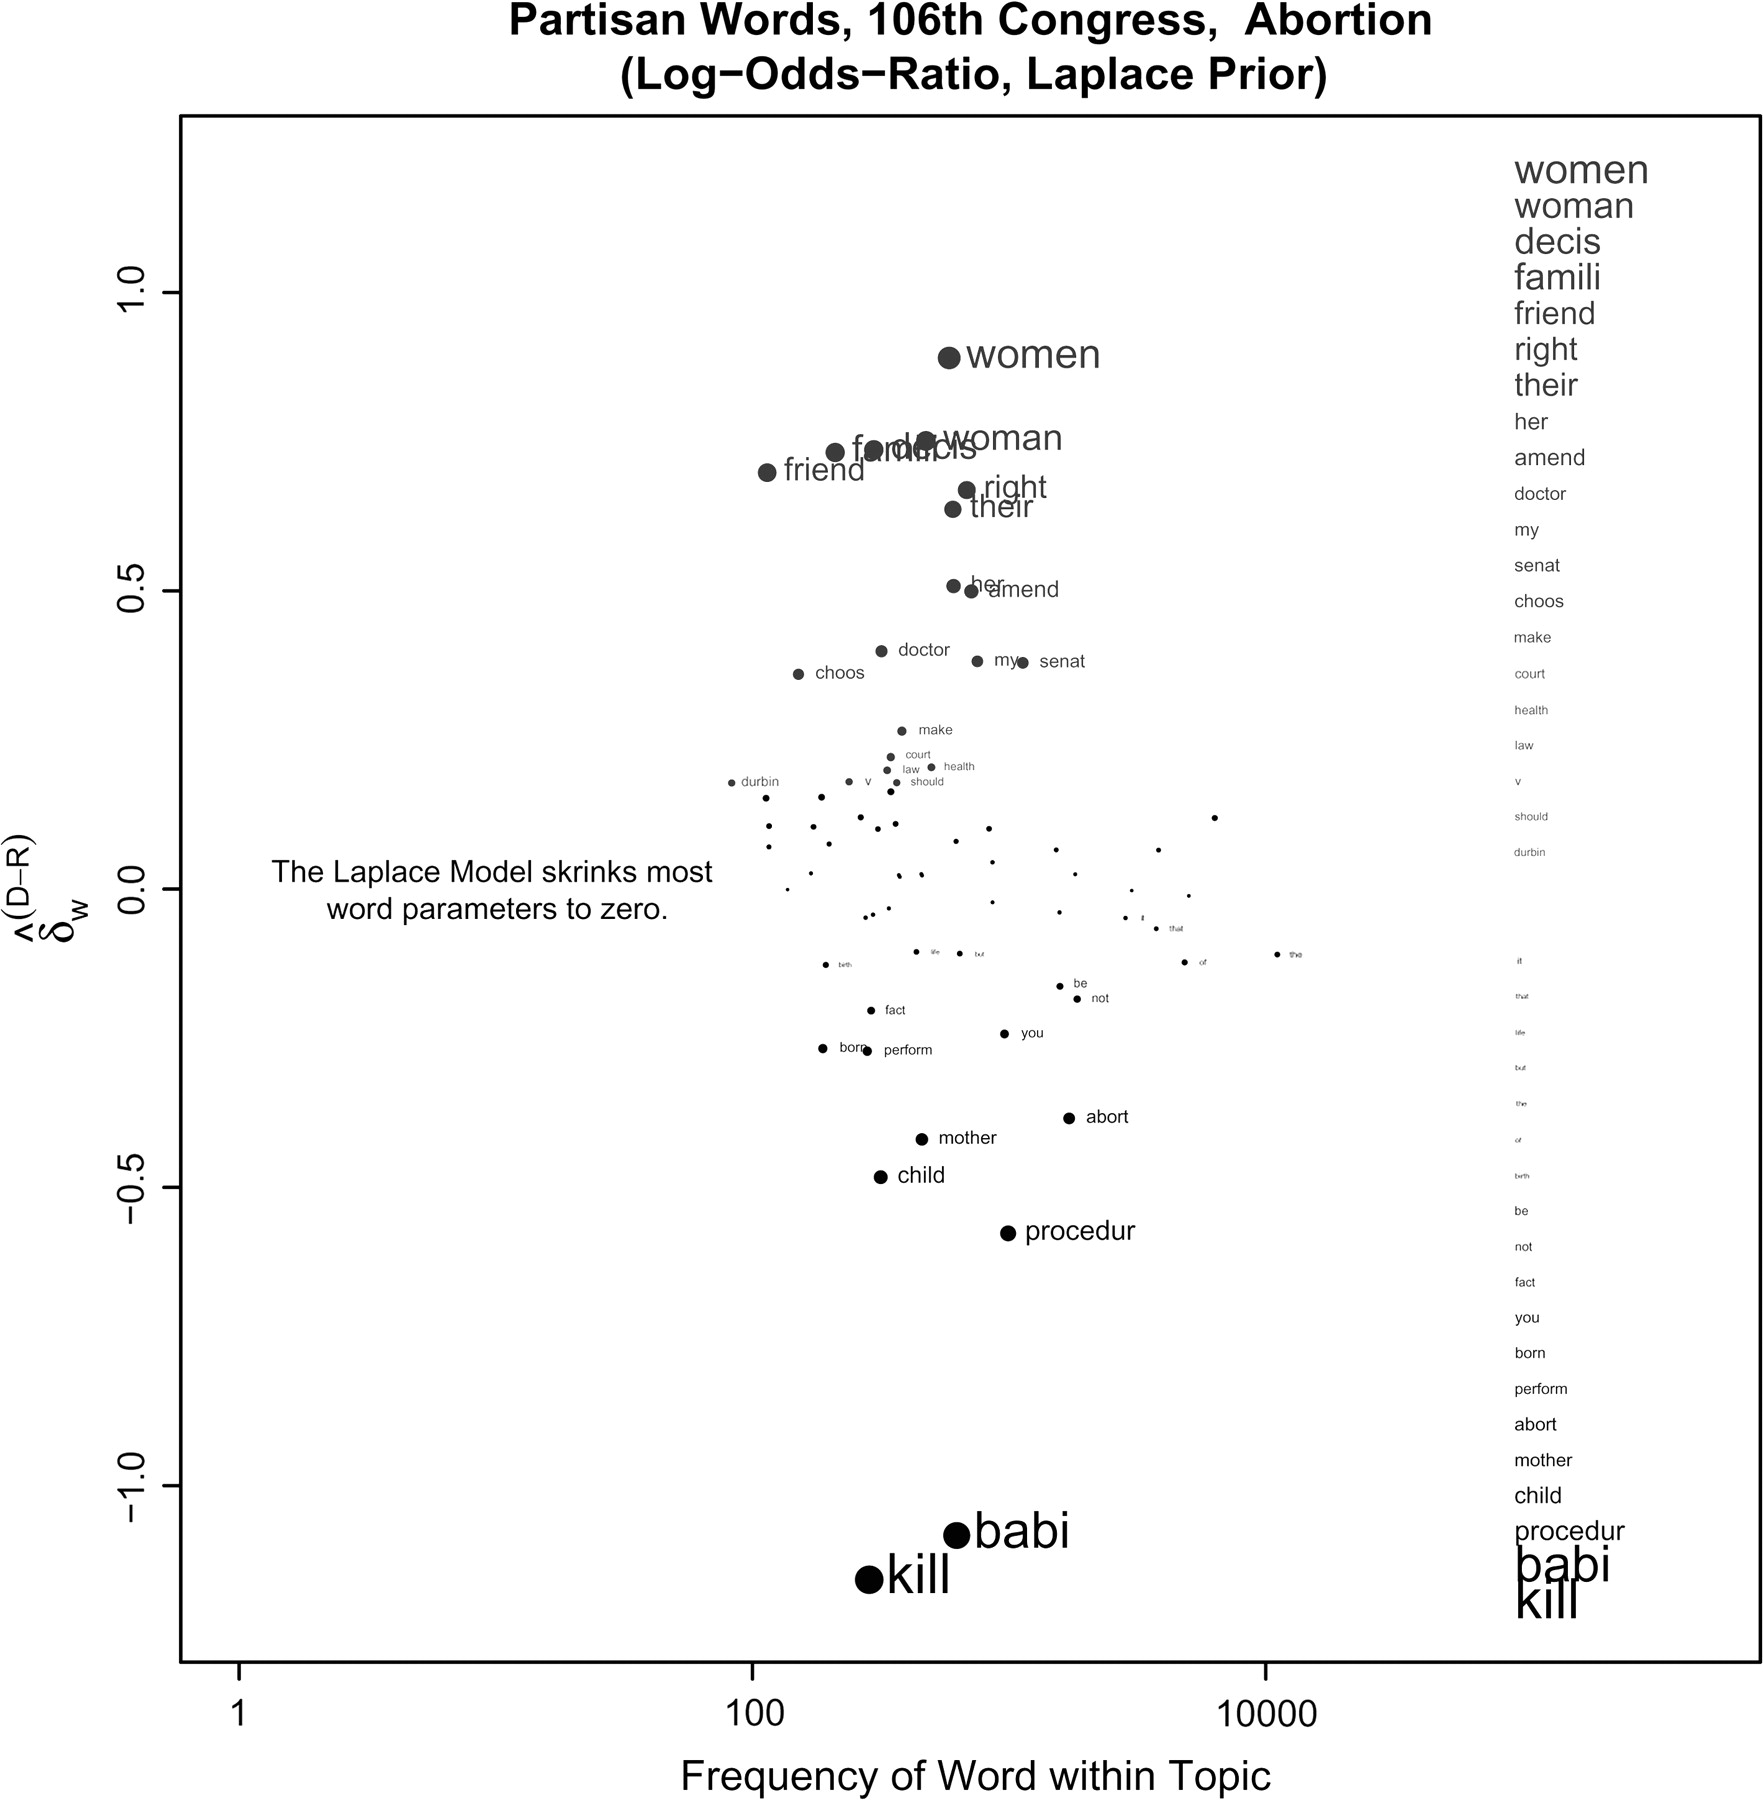
\includegraphics[scale=.1]{pictures/fightin1}}
%{\footnotesize An additional prior means that words whose partisanship is not clear will receive partisan contrasts that are exactly zero. Identifying %important words is now easier (Monroe et al. 2009).}
%\end{frame}


%\begin{frame}[t,fragile]\frametitle{Lexical Instability}
%\centerline{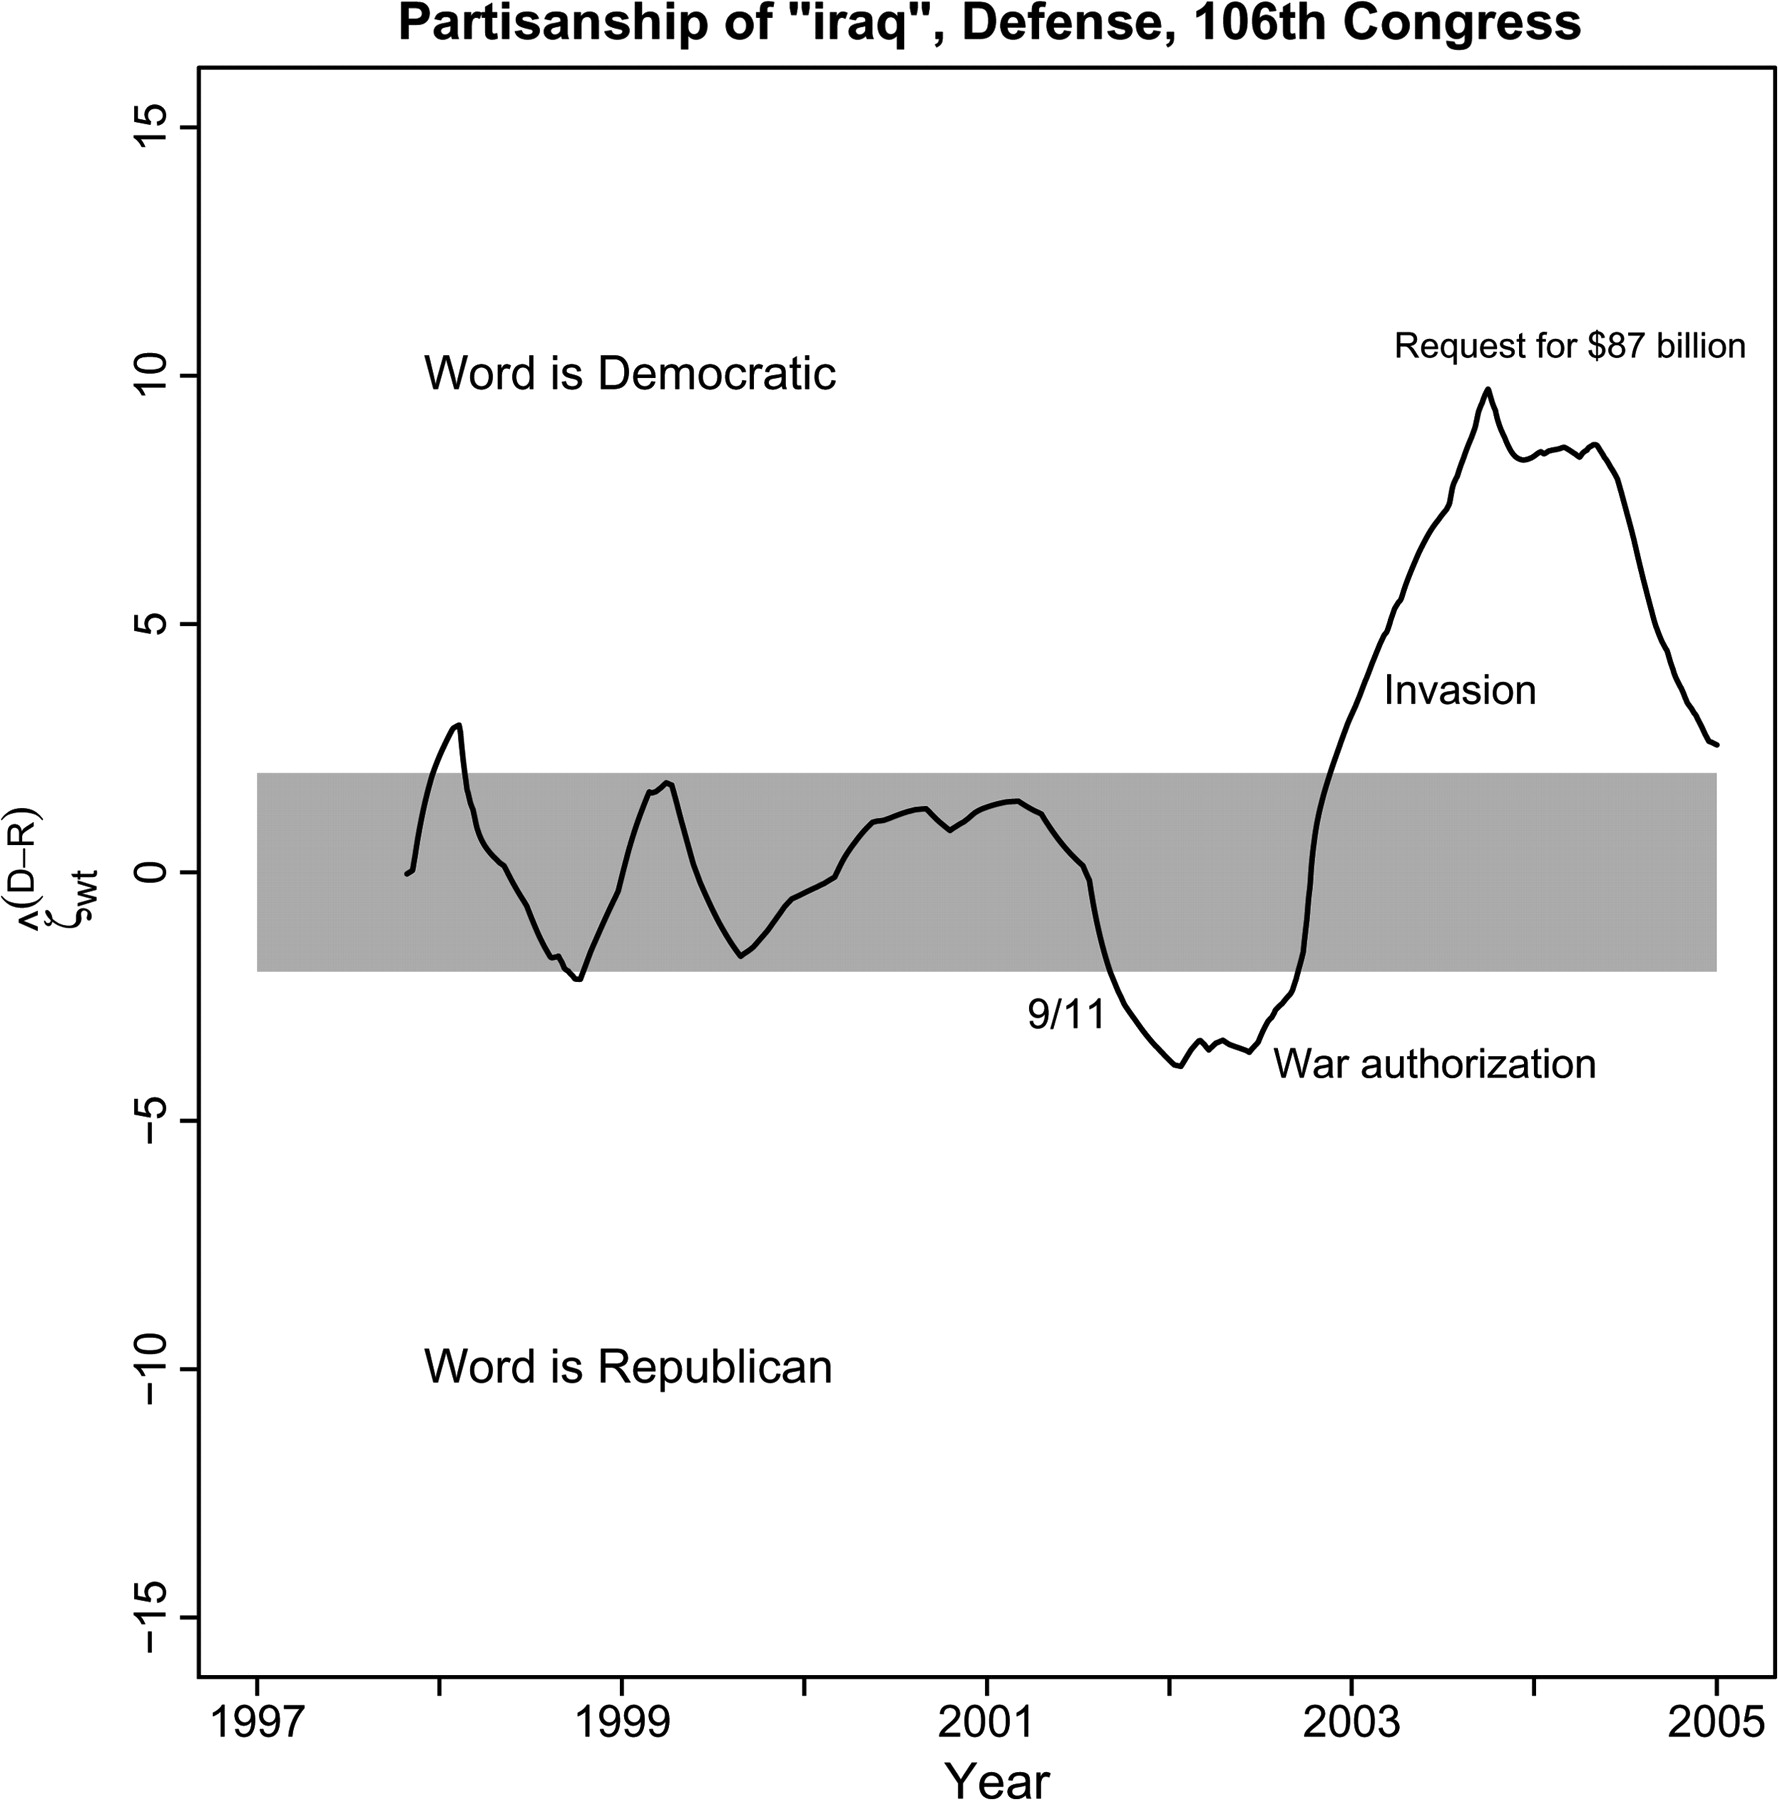
\includegraphics[scale=.1]{pictures/fightin2}}
%\end{frame}



%\begin{frame}[t,fragile]\frametitle{Classification: Good Old Logit}
%i%t is tempting to go with methods we know (disciminative style)
%\begin{eqnarray*}
%\hat{\theta}_{k|w} &=& P(Z=k \mid W_1 \ldots W_V)\\
%&=& \text{logit}^{-1}(\alpha + \beta_1 W_1 + \beta_2 W_2 + \ldots)
%\end{eqnarray*}
%This is a bad idea
%\ita
%\itm Why?
%\itz
%\end{frame}

%\begin{frame}[t,fragile]\frametitle{Bad Old Logit}
%The number of word types V is almost much larger than the number of documents D
%\ita
%\itm Many more `cases' than `variables'
%\itm \textit{and} no constraint on possible solutions
%\itz
%We need \textit{serious} regularisation\ldots
%\end{frame}



\begin{frame}[t,fragile]\frametitle{Latent Dirichlet Allocation}
What if documents don't belong to only one category?
\ita
\itm Each document is a mixture over topics
\itm Each topic is a mixture over words
\itz
Using LDA gives us:
\ita
\itm Distribution of words for each topic ($\beta$)
\itm Proportion of a document in each topic ($\theta$)
\itz
Setting up LDA
\ita
\itm Still uses bag of words
\itm Number of topics fixed ex ante
\itm Topics examined ex post --- unsupervised learning
\itz
\end{frame}



\begin{frame}[t,fragile]\frametitle{Visualizing Topic Models}
%\vspace{10 mm}
\centerline{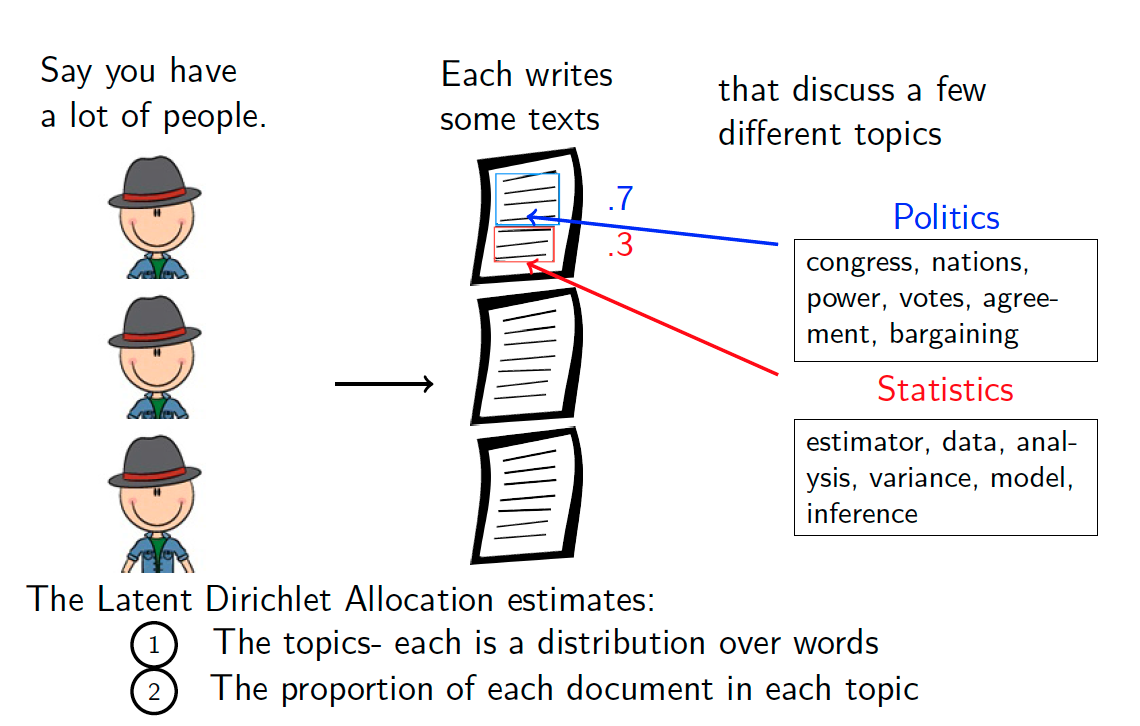
\includegraphics[scale=.27]{pictures/ldavis.png}}
\centerline{\normalsize Courtsey of Brandon Stewart}
\end{frame}


\begin{frame}[t,fragile]\frametitle{Latent Dirichlet Allocation Components}
Given dimensions:
\ita
\item \textbf{N} documents, \textbf{J} different topics, \textbf{K} unique words
\itz
We want the following matrices:
\ita
\item $X = N \times K$ document-term matrix (observed)
\item $\theta = N \times K$ matrix with row $\theta_i = (\theta_{i1},\ldots,\theta_{iK})$
  \ita
  \item $\theta_{ik}$: Proportion of document $i$ allocated to topic $k$
  \itz
\item $\beta = K \times J$ matrix with row $\beta_k = (\beta_{k1}, \ldots, \beta_{kJ})$
  \ita
  \item $\beta_{kj}$: Probability of using word J, if topic k is chosen
  \itz
\item $\alpha$ = K length population prior for $\theta$
\itz
Objective function: f(X, $\beta, \theta, \alpha)$
\end{frame}


\begin{frame}[t,fragile]\frametitle{LDA Generative Model}
When writing a word ($m$) for document $i$:
\begin{align*}
\only<1>{
\text{p}(\theta_i | \alpha) &= \text{Dirichlet}(\alpha) && \text{(Pick potential topics $\theta_i$)}\\
}
\text{p}(z_{im} | \theta_i)  &= \text{Multinomial}(1, \theta_i) && \text{ (Pick the topic z to discuss)}\\
x_{im} | \beta_k, z_{im} &= \text{Multinomial}(1, \beta_k)  && \text{ (Pick a word from topic $z_{im}$) }\\
\text{p}(\beta_k) &= \text{Dirichlet}(\eta)  && \text{(Prior on topics)}\\
%\text{p}(\alpha_k) &= \text{Gamma}(\alpha,\beta)  && \text{(Prior on document proportions)}
\end{align*}

with

p($\beta$, $\theta$, Z, $\alpha$ | X) $\propto$  p($\beta$ | $\eta$) $\cdot$ p($\theta$|$\alpha$) $\cdot$ p(Z | $\theta$) $\cdot$ p(X | $\beta$, Z)
\end{frame}


\begin{frame}[t,fragile]\frametitle{Generative vs discriminative training}
\vspace{2cm}
\centerline{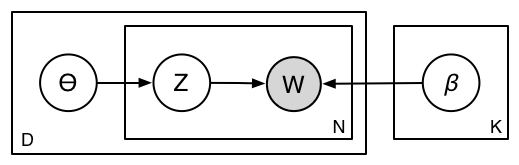
\includegraphics[scale=.6]{pictures/new-topics-ca.png} }
\vfill
\end{frame}



\begin{frame}[t,fragile]\frametitle{Intuition on LDA}
p($\beta$, $\theta$, Z, $\alpha$ | X) $\propto$  p($\beta$ | $\eta$) $\cdot$ p($\theta$|$\alpha$) $\cdot$ p(Z | $\theta$) $\cdot$ p(X | $\beta$, Z)

Remember rows of $\beta$ and $\theta$ must sum to 1!

p(X | $\beta$, Z): Favors co-occurring words, segregated topics
\ita
\item $\beta$ = (0.5,0.5,0,0) vs $\beta$ = (0.25,0.25,0.25,0.25)
 \itz

p(Z | $\theta$): Higher if $\theta$ is concentrated (i.e. fewer potential topics)
\ita
\item $\theta$ = (0.5,0.5, 0, 0) vs. $\theta$ = (0.25, 0.25, 0.25, 0.25) 
\itz

Joint distribution favors sparse topics, small topic clusters

But data often need a larger number of topics to assign small topic clusters to data


\end{frame}


%SNTV-MMD: Single nontransferable vote, multimember district
%More competition within party, as majority-seeking parties run multiple candidates in each district
% MMM: Mixed member district: PR + single member districts

\begin{frame}[t,fragile]\frametitle{Japanese Campaign Manifestos (Catalinac 2016)}
Examines the effect of electoral reform
\ita
\itm Before 1994: SNTV-MMD (more intraparty competition)
\itm After 1994: Mixed member majoritarian (PR + SMD)
\itz
LDA on N=7497 candidate manifestos for Diet 1950-2009
\ita
\itm Hand transcribed, OCR failed
\itm More complicated in Japanese
\itz
Characterizing campaigns across 50+ years
\ita
\itm What do candidates talk about?
\itm How did electoral reform change incentives?
\itm Why increasing interest in militaristic foreign action? 
\itz
\end{frame}

\begin{frame}[t,fragile]\frametitle{Japanese Manifestos}
\vspace{10 mm}
\centerline{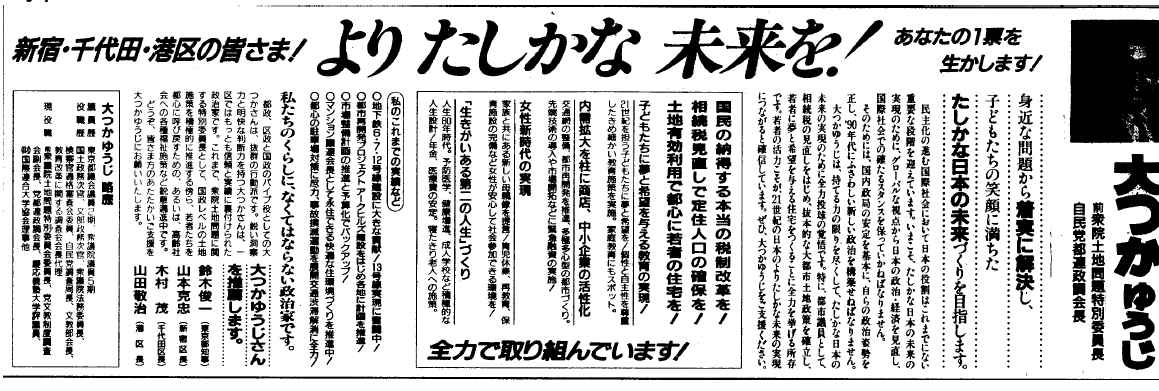
\includegraphics[scale=.27]{pictures/jpmanifesto.png}}
%\centerline{\normalsize In LDA, each document can contain multiple topics}
\end{frame}


\begin{frame}[t,fragile]\frametitle{Japanese Manifesto Topics}
\vspace{10 mm}
\centerline{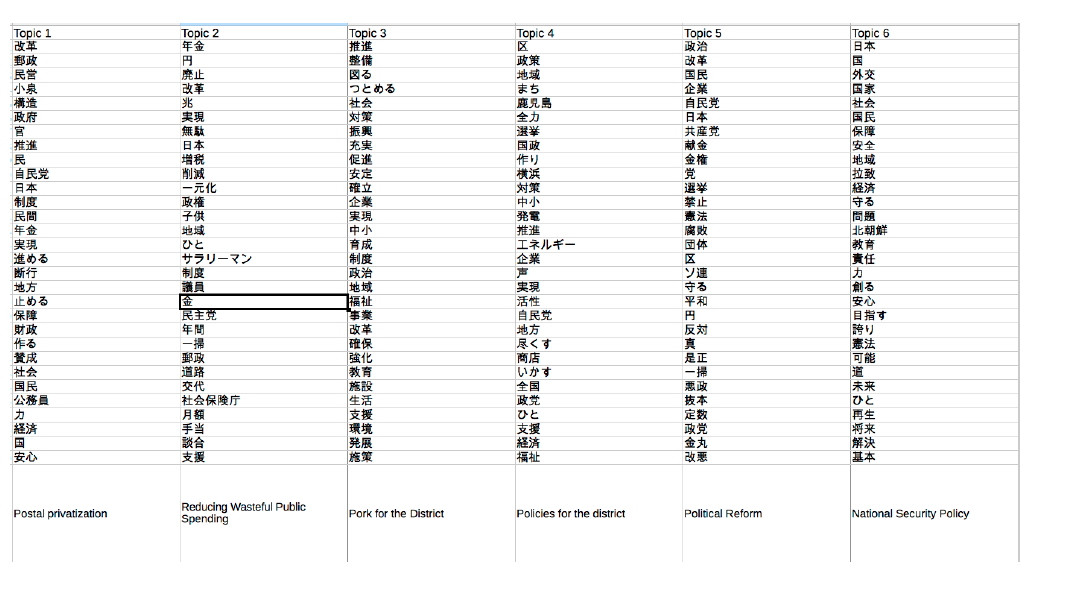
\includegraphics[scale=.27]{pictures/jptopic.png}}
%\centerline{\normalsize In LDA, each document can contain multiple topics}
\end{frame}


\begin{frame}[t,fragile]\frametitle{Manifesto Content over Time}
\vspace{10 mm}
\centerline{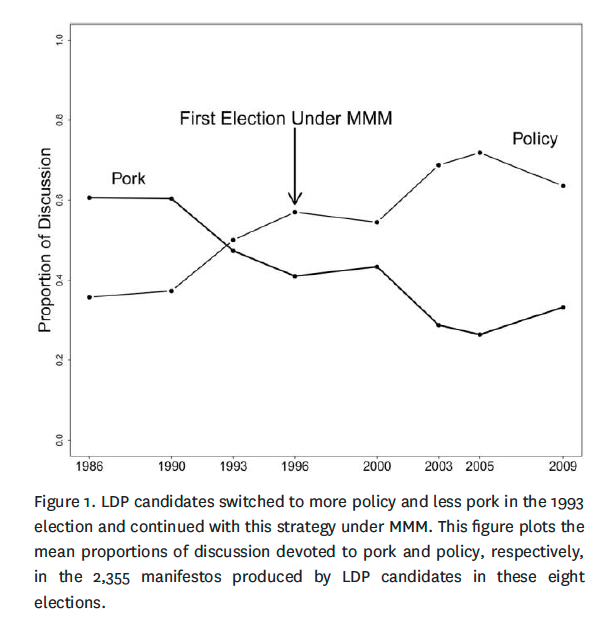
\includegraphics[scale=.27]{pictures/jpcontent.png}}
%\centerline{\normalsize In LDA, each document can contain multiple topics}
\end{frame}


\begin{frame}[t,fragile]\frametitle{Foreign Policy Content}
\vspace{10 mm}
\centerline{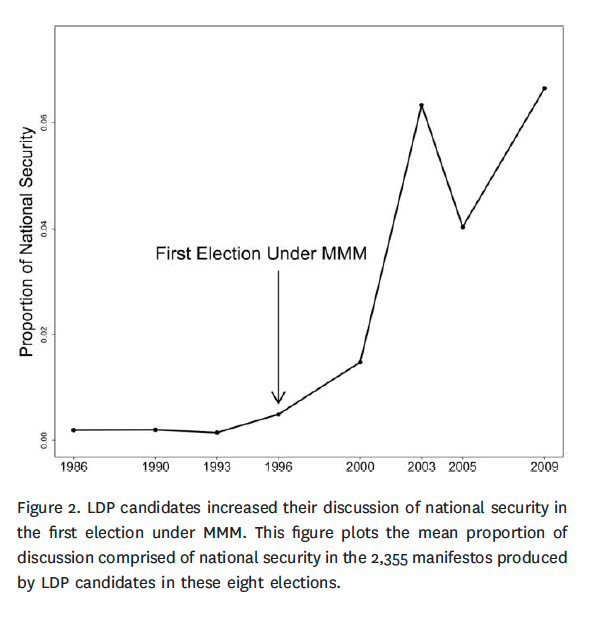
\includegraphics[scale=.27]{pictures/jpforeign.png}}
%\centerline{\normalsize In LDA, each document can contain multiple topics}
\end{frame}




\begin{frame}[t,fragile]\frametitle{Wrapping up}
For single category classification
\ita
\itm Discriminative: Model $P(Z \mid \{W\}, \beta) = \theta_{z|w}$ directly
\itm Generative: Model $P(\{W\} \mid Z, \beta)$ and $P(Z)=\theta_z$, then get $P(Z \mid \{W\}, \beta) = \theta_{z|w}$ via Bayes theorem
\itz
For multiple categories
\ita
\itm Latent Dirichlet Allocation
\itm More generally used for discovery of topics
\itz
Tomorrow's Lab
\ita
\itm Classifying NY Times articles by topic
\itz
\end{frame}

\end{document}




